% Chapter 11. One request through a stateless server.
\documentclass[tikz,border=6pt]{standalone}
% Shared look for every TikZ figure in the book.
% Colours match book/preamble.tex exactly. Change both or neither.

\usepackage{tikz}
\usepackage{xcolor}
\usepackage{amsmath}
\IfFileExists{libertinus.sty}{\usepackage[mono=false]{libertinus}}{}
\IfFileExists{inconsolata.sty}{\usepackage[varqu,varl,scaled=0.95]{inconsolata}}{}

\usetikzlibrary{
  arrows.meta, positioning, calc, fit, backgrounds, shapes.geometric,
  shapes.misc, decorations.pathreplacing, decorations.pathmorphing,
  patterns, chains, matrix, shadows.blur
}

\definecolor{ink}{HTML}{15181D}
\definecolor{muted}{HTML}{5B6472}
\definecolor{rule}{HTML}{C9CED6}
\definecolor{wash}{HTML}{F4F5F7}
\definecolor{accent}{HTML}{0F5C8C}
\definecolor{accentsoft}{HTML}{E7F0F6}
\definecolor{warm}{HTML}{B4531A}
\definecolor{warmsoft}{HTML}{FBF0E7}
\definecolor{good}{HTML}{2C6E49}
\definecolor{goodsoft}{HTML}{E9F2EC}
\definecolor{danger}{HTML}{9B2226}
\definecolor{dangersoft}{HTML}{FAECEC}

\tikzset{
  font=\sffamily\small,
  >={Stealth[length=5pt, width=4pt]},
  %
  box/.style={
    draw=rule, line width=0.8pt, fill=wash, rounded corners=2pt,
    inner sep=7pt, align=center, text=ink, minimum height=9mm,
  },
  boxa/.style={box, draw=accent, fill=accentsoft},
  boxg/.style={box, draw=good,   fill=goodsoft},
  boxw/.style={box, draw=warm,   fill=warmsoft},
  boxd/.style={box, draw=danger, fill=dangersoft},
  %
  lane/.style={draw=rule, line width=0.7pt, fill=white, rounded corners=2pt,
               inner sep=6pt, align=center, minimum width=26mm},
  %
  flow/.style={draw=accent, line width=1.0pt, ->},
  flowback/.style={flow, densely dashed},
  flowmuted/.style={draw=muted, line width=0.8pt, ->},
  lifeline/.style={draw=rule, line width=0.7pt, densely dotted},
  %
  lbl/.style={font=\sffamily\scriptsize, text=muted, inner sep=2pt},
  lblink/.style={font=\sffamily\scriptsize, text=ink, inner sep=2pt},
  tag/.style={font=\ttfamily\scriptsize, text=accent, inner sep=2pt,
              fill=white, inner xsep=3pt},
  note/.style={font=\sffamily\scriptsize\itshape, text=muted, align=left},
  %
  band/.style={draw=none, rounded corners=1pt},
  tick/.style={draw=muted, line width=0.6pt},
}

% A horizontal timeline bar segment: \barseg{x0}{x1}{y}{colour}{label}
\newcommand{\barseg}[5]{%
  \fill[#4, rounded corners=1pt] (#1,#3-0.16) rectangle (#2,#3+0.16);
  \node[lbl, text=white, font=\sffamily\scriptsize\bfseries]
       at ({(#1+#2)/2},#3) {#5};
}

\begin{document}
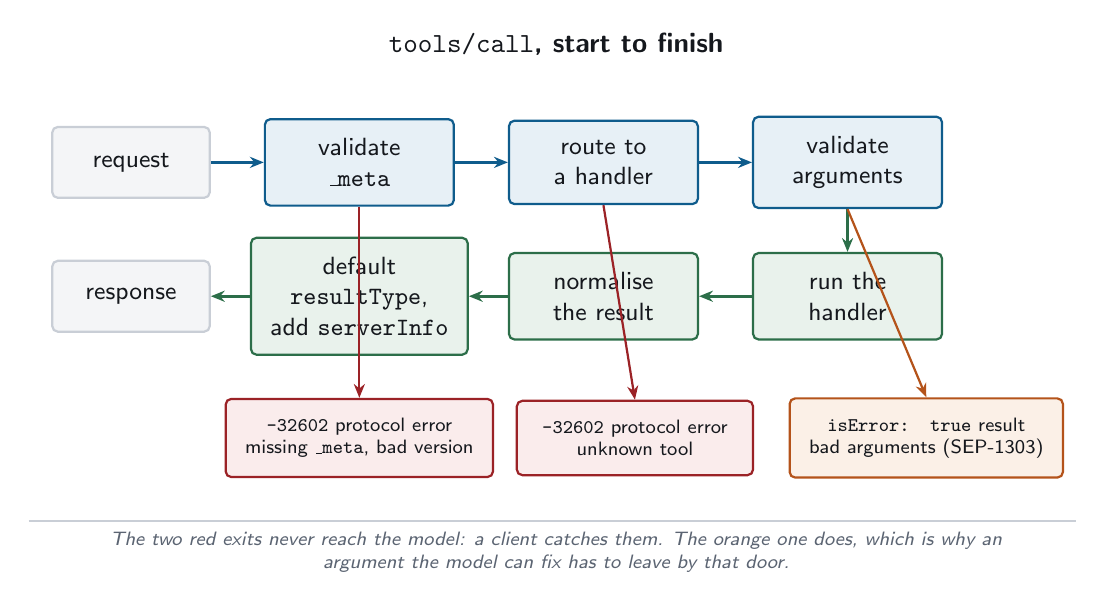
\begin{tikzpicture}[x=1cm, y=1cm, node distance=0pt]

  \node[lblink, font=\sffamily\bfseries] at (5.4,3.5) {\texttt{tools/call}, start to finish};

  \node[box, minimum width=20mm] (in) at (0,2.0) {request};
  \node[boxa, minimum width=24mm] (env) at (2.9,2.0) {validate\\\texttt{\_meta}};
  \node[boxa, minimum width=24mm] (route) at (6.0,2.0) {route to\\a handler};
  \node[boxa, minimum width=24mm] (args) at (9.1,2.0) {validate\\arguments};

  \draw[flow] (in) -- (env);
  \draw[flow] (env) -- (route);
  \draw[flow] (route) -- (args);

  \node[boxg, minimum width=24mm] (run) at (9.1,0.3) {run the\\handler};
  \node[boxg, minimum width=24mm] (norm) at (6.0,0.3) {normalise\\the result};
  \node[boxg, minimum width=24mm] (meta) at (2.9,0.3) {default\\\texttt{resultType},\\add \texttt{serverInfo}};
  \node[box, minimum width=20mm] (out) at (0,0.3) {response};

  \draw[flow, draw=good] (args) -- (run);
  \draw[flow, draw=good] (run) -- (norm);
  \draw[flow, draw=good] (norm) -- (meta);
  \draw[flow, draw=good] (meta) -- (out);

  % failure exits
  \node[boxd, minimum width=30mm, font=\sffamily\scriptsize] (e1) at (2.9,-1.5)
    {\texttt{-32602} protocol error\\{\scriptsize missing \texttt{\_meta}, bad version}};
  \node[boxd, minimum width=30mm, font=\sffamily\scriptsize] (e2) at (6.4,-1.5)
    {\texttt{-32602} protocol error\\{\scriptsize unknown tool}};
  \node[boxw, minimum width=32mm, font=\sffamily\scriptsize] (e3) at (10.1,-1.5)
    {\texttt{isError: true} result\\{\scriptsize bad arguments (SEP-1303)}};

  \draw[flowmuted, draw=danger] (env.south) -- (e1.north);
  \draw[flowmuted, draw=danger] (route.south) -- (e2.north);
  \draw[flowmuted, draw=warm] (args.south) -- (e3.north);

  \draw[rule, line width=0.7pt] (-1.3,-2.55) -- (12.0,-2.55);
  \node[note, align=center, text=muted] at (5.4,-2.95)
    {The two red exits never reach the model: a client catches them.
     The orange one does, which is why an\\argument the model can fix
     has to leave by that door.};

\end{tikzpicture}
\end{document}
